\documentclass[a4paper, 8pt, twocolumn]{article}

% Font includes
\usepackage[T1]{fontenc}
\usepackage[utf8]{inputenc}

% Document geometry
\usepackage[left=2cm, right=2cm]{geometry}

% Plots and tables
\usepackage{graphicx}
\usepackage{subfig}
\usepackage{tabularx}

% Math includes
\usepackage{amsmath}
\usepackage{amsfonts}

% Listing includes
\usepackage{minted}

% References & Hyperrefs
\usepackage{cleveref}
\usepackage{hyperref}

% Affiliate includes
\usepackage{authblk}

% Custom commands
\newcommand{\sref}[1]{Section \ref{#1}}

% Title
\title{A Twitter based Brexit analysis}
\author[1]{J. Kunath}
\author[2]{J. Gacon}
\author[3]{Dr. I. Moise}
\affil[1]{Department of Physics, ETH Zurich}
\affil[2]{Department of Mathematics, ETH Zurich}
\affil[3]{Department of Humanities, Social and Political Sciences, ETH Zurich}

\begin{document}

%%! Title 
\maketitle

%%! Abstract
\twocolumn[
  \begin{@twocolumnfalse}
    \begin{abstract}
      The politics in Europe recently are subject to changes that are heavily biased towards the right wing and conservatives. 
      Scenarios which we deem unthinkable occur surprisingly often, the most prominent examples being the so-called ``Brexit'' and the Trump administration. 
      They all share far-reaching similarities:
      A dedicated political group pursuing a controversial goal and an initially low attention of the opposition.  
      Voters that feel left behind and forgotten see their opportunity to have an impact. The election divides the country. 

      We are interested in how the attention for such political events fluctuates over time. 
      As a case study we chose the Brexit and as measure of attention the activity on related topics on Twitter.  \\ \\
    \end{abstract}
    \mbox{}
  \end{@twocolumnfalse}
]


%%! Text
\section{Introduction}

Twitter provides Tweet data from the last 7 days in the REST API \cite{rest-api}. 
The Brexit has risen a lot of attention in the last few weeks so we can investigate the activity on Twitter very well. 
We were crawling data from the API for several time windows between April 5th and May 10th 2017. Also we had access to Twitter archives from the Computational Social Science group at ETH,
which allowed us to get Tweets from February, April and May 2016.

We used a set of Brexit-related keywords to filter for relevant input. Using the time-zone as location of the tweet we can restrict the search to Great Britain. 
As a tool for analysing the useful sources, we used two tools: Python's Vader sentiment analysis and our own sentiment analysis, based on the Brexit gold standard 
- a 2000 Tweets database whose sentiments have been assigned manually by an expert group.

We will investigate the activity of Tweets in favour and against the Brexit, identify peaks and interesting behaviours and try to map those to political events. 
This way we will see, if the interest in politics of certain groups follows an explainable behaviour.

In \sref{sec:sentiment-analysis} we explain our approach sentiment analysis approach in detail. 
We continue in \sref{sec:frequency-analysis} by looking at the frequency of keywords over time in different regions.
Specifications about the implementations can be found in \sref{sec:implementations} and finally we present the
results in \sref{sec:results}.


\section{Sentiment analysis}\label{sec:sentiment-analysis}
%
% TODO
%
Djonaaas

\section{Frequency analysis}\label{sec:frequency-analysis}
%
% TODO 
%
To see how the attention of the Brexit evolves over time we investigated how often certain keywords appeared.
The timestamp is available in every tweet and is easily accessable.
For the location the tag \texttt{geo} of \texttt{place} turned out not be useful as by far most tweets have the location disabled.
However we the \texttt{user\_time\_zone} is contained in almost all our data, which does the job in our case. 
Timezone does not indicate the UTC$\pm$HH:MM only, but actually tells you the nearest example city of this time zone.
A typical dataset would read:
\newline\newline
{\ttfamily
  \begin{tabular}{|l|l|l|}
    \hline
    created\_at & geo & user\_time\_zone \\ \hline
    2017-04-02 23:19:42 & None & None \\ \hline
    2017-04-02 23:19:45 & None & Karachi \\ \hline
    2017-04-02 23:19:46 & None & London \\ \hline
    2017-04-02 23:19:52 & None & Moscow \\ \hline
  \end{tabular}
}
\newline\newline
From a testset of 1067045 tweets, 17909 (1.7\%) had a \texttt{place} tag, 631172 (59\%) a \texttt{user\_time\_zone} and 0 a geolocation.

Now one simply needs to filter the tweets according to wanted timezones and keywords, group them by day and count.
Results using the timezone filter London and multiple keywords are shown in \cref{fig:frequency-london} and the total 
activity in \cref{fig:frequency-tot}.

\begin{figure*}[h]
  \subfloat[We counted the appearance of certain keywords in the tweets for each day in our data.
            Words like ``ukip'' are very present over the whole time window. We excluded the keyword ``brexit'',
            as it is included in almost every Tweet.\label{fig:frequency-london}]{
              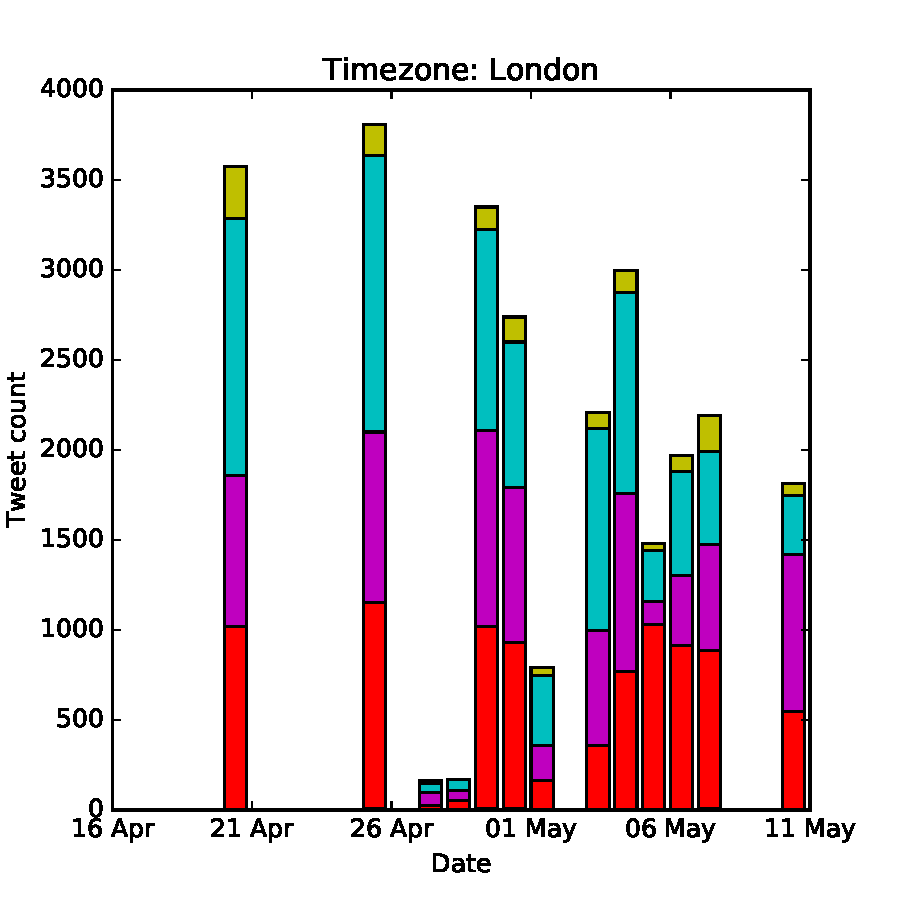
\includegraphics[width=0.48\linewidth]{../frequency_stacked_London.pdf}
            }
  \hfill
  \subfloat[Total activity of Brexit-related tweets. As one can see almost all Tweets contain the keyword ``brexit'',
            thus it cannot be used to classify sentiments. However it is very useful to roughly filter for Tweets about
            the referendum.\label{fig:frequency-tot}]{
              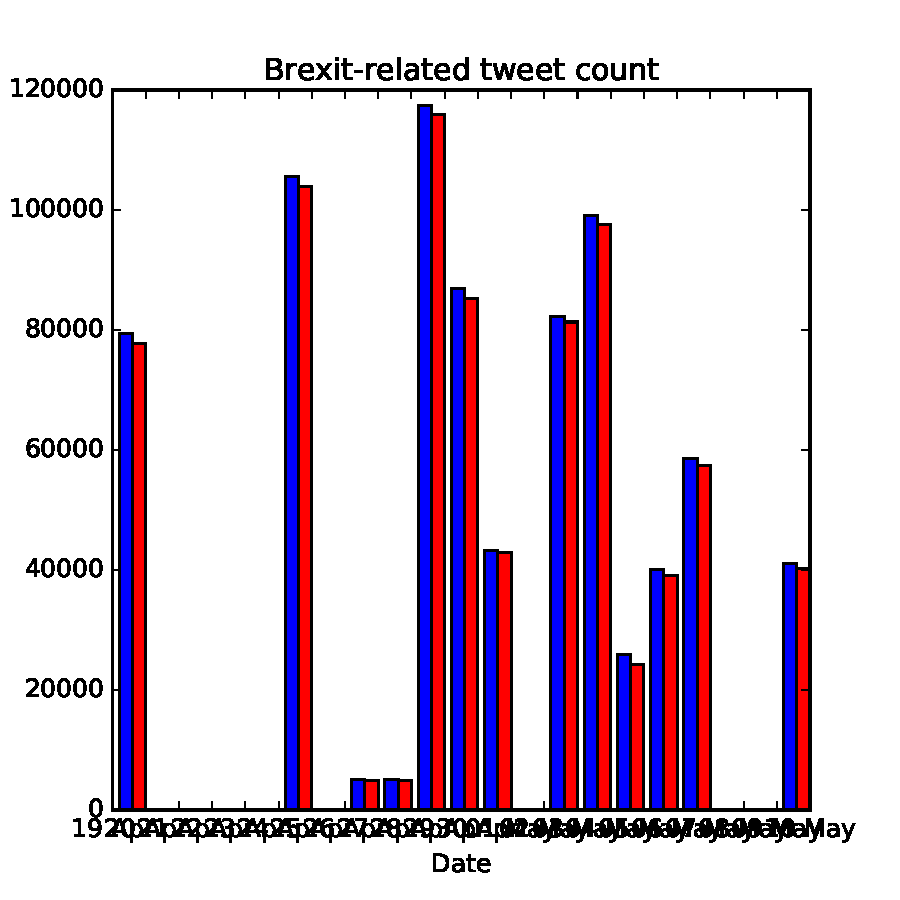
\includegraphics[width=0.48\linewidth]{../frequency_brexit.pdf}
            }
  \caption{Frequency analysis}
\end{figure*}


\begin{figure}[hp]
  \centering
  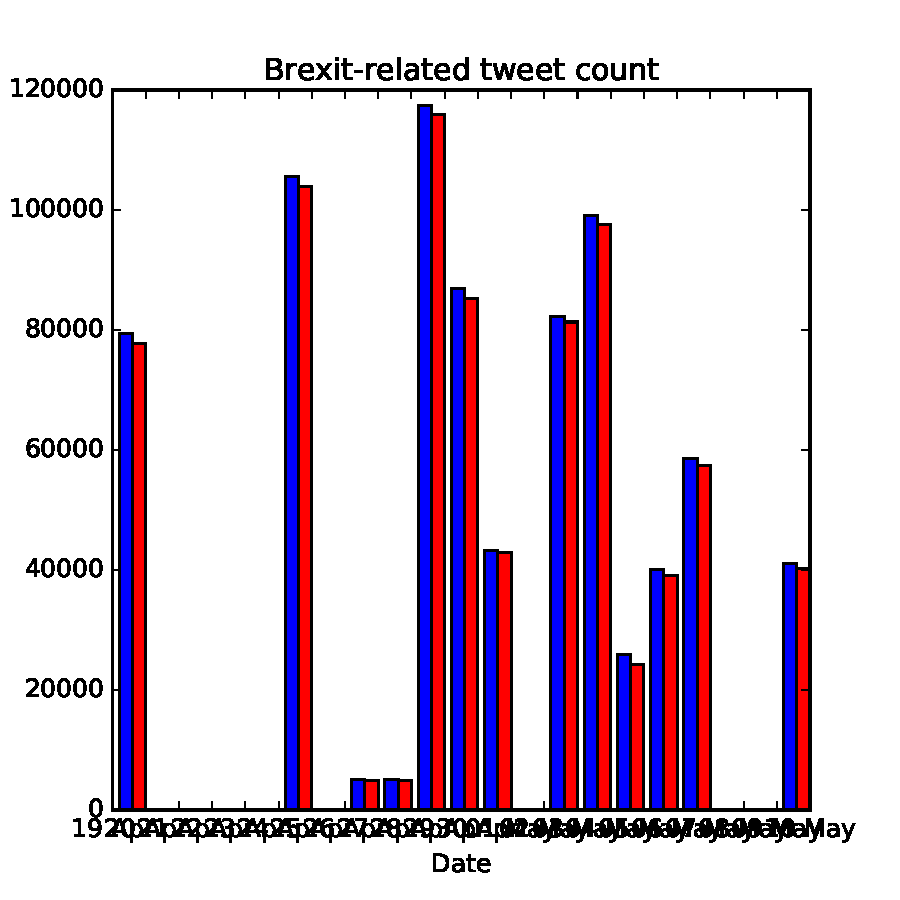
\includegraphics[width=\linewidth]{../frequency_brexit.pdf}
  \caption{Total activity of Brexit-related tweets. As one can see almost all Tweets contain the keyword ``brexit'',
           thus it cannot be used to classify sentiments. However it is very useful to roughly filter for Tweets about
           the referendum.}
\end{figure}

\section{Implementations}\label{sec:implementations}
%
% TODO
%
Beideeeee

\section{Results}\label{sec:results}
%
% TODO
%
Beideeee

%%! Bibliography
\begin{thebibliography}{9} % 9 --> up to 9 references, 99 --> up to 99 references (gives no. digits)

  \bibitem{rest-api}
    Twitter REST API, 
    \url{https://dev.twitter.com/rest/public/search}

\end{thebibliography}

\end{document}
